\section{HYCYMODEL (model ID: 42)}
The HYCYMODEL (fig.~\ref{fig:00_schematic}) is originally developed for use in heavily forested catchments in Japan \citep{Fukushima1988}. The original model specifies evaporation from the $S_b$ store as $E_T = e_p(i)*Q_b/Q_{bc}, \text{ if } S_u < 0 ~\&~ S_b < S_{bc}$, with $Q_{bc} = f(S_{bc})$. However, no further details are given and $S_{bc}$ is not listed as a parameter. We assume that $S_{bc}$ [mm] is a threshold  parameter and that evaporation potential declines linearly to zero when the store drops under this threshold. The model has 6 stores and 12 parameters ($C$, $I_{1,max}$, $\alpha$, $I_{2,max}$, $k_{in}$, $D_{50}$, $D_{16}$, $S_{bc}$, $k_b$, $p_b$, $k_h$ and $k_c$). The model aims to represent:

\begin{itemizecompact}
\item Split between channel and ground precipitation;
\item Interception by canopy and stems/trunks;
\item Overland flow from a variable contributing area;
\item Non-linear channel flow, hillslope flow and baseflow;
\item Channel evaporation.
\end{itemizecompact}

\subsection{MARRMoT model name}
m\_42\_hycymodel\_12p\_6s \\

% Equations
\subsection{Model equations}

% Model layout figure
{ 																	% This ensures it doesn't warp text further down
\begin{wrapfigure}{l}{7cm}
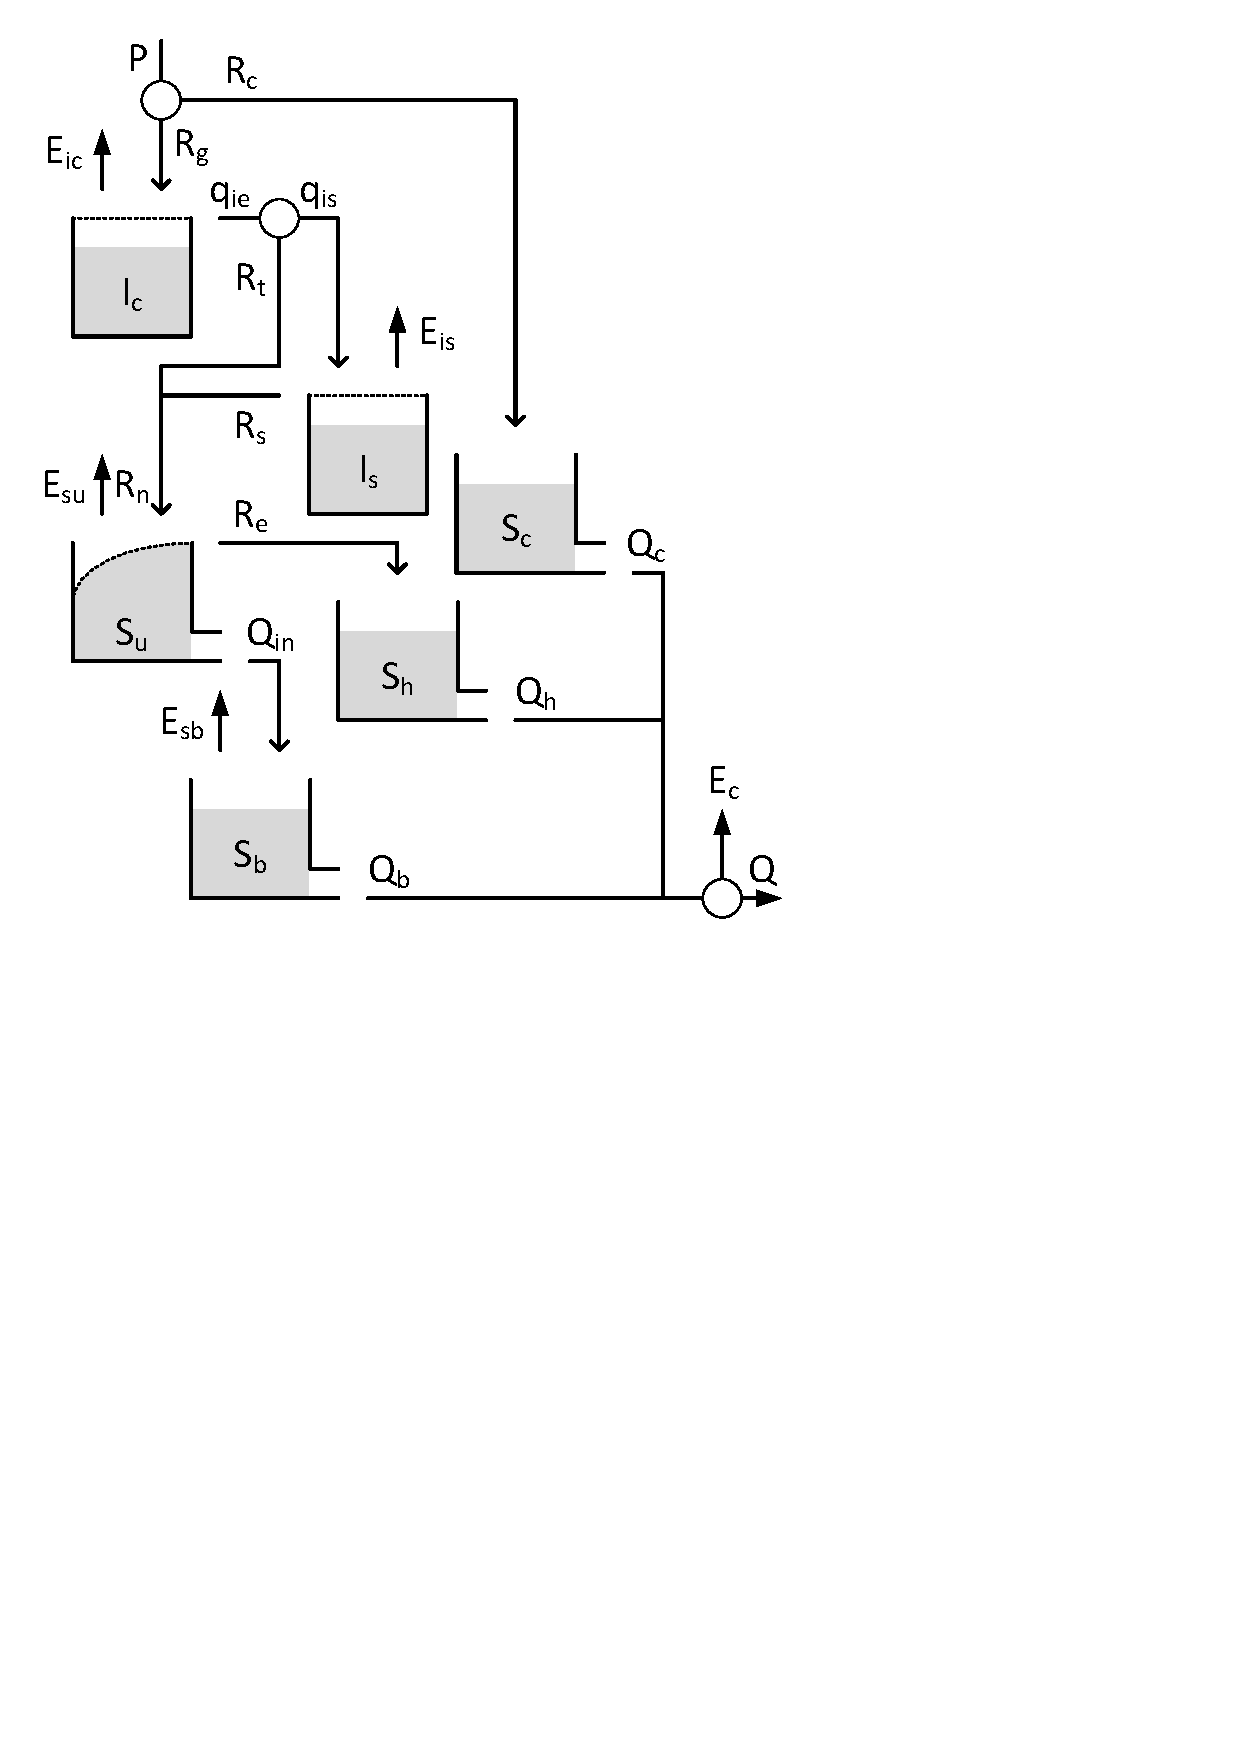
\includegraphics[trim=1cm 14.5cm 7cm 1cm,width=7cm,keepaspectratio]{./AppA_files/42_schematic.pdf}
\caption{Structure of the HYCYMODEL} \label{fig:00_schematic}
\end{wrapfigure}

\begin{align}
	\frac{dI_c}{dt} &= R_g-E_{ic} -q_{ie} \\
	R_g &= (1-C)P\\
	E_{ic} &= 
	\begin{cases}
		(1-C)*E_p, & \text{if } I_c > 0 \\
		0, & \text{otherwise}
	\end{cases}\\
	q_{ie} &= 	\begin{cases}
		R_g, & \text{if } I_c = I_{1,max} \\
		0, & \text{otherwise}
	\end{cases}
\end{align}

Where $I_c$ [mm] is the current canopy storage, refilled by rainfall on ground $R_g$ $[mm/d]$ and drained by evaporation $E_{ic}$ $[mm/d]$ and canopy interception excess $Q_{ie}$ $[mm/d]$.
$R_g$ is the fraction (1-C) [mm] of rainfall $P$ $[mm/d]$ that falls on ground (and not in the channel).
This fraction appears several times in the model to scale evaporation values according to surface area.

} % end of wrapfigure fix

\noindent$E_{ic}$ occurs at the potential rate $E_p$ $[mm/d]$ when possible.
$q_{ie}$ only occurs when the canopy store is at maximum capacity $I_{1,max}$ [mm].

\begin{align}
	\frac{dI_s}{dt} &= q_{is} - E_{is}  - R_s\\
	q_{is} &= \alpha*q_{ie} \\
	E_{is} &= \begin{cases}
		(1-C)*E_p, &\text{if } I_s > 0 \\
		0, &\text{otherwise} \\
	\end{cases} \\
	R_s &= \begin{cases}
		q_{is}, &\text{if } I_s = I_{2,max}\\
		0, &\text{otherwise}\\
	\end{cases}	
\end{align}

Where $I_s$ [mm] is the current stem and trunk storage, refilled by a fraction of canopy excess $q_{is}$ $[mm/d]$ and drained by evaporation $E_{is}$ $[mm/d]$ and stem flow $R_s$ $[mm/d]$.
$q_{is}$ is the fraction $\alpha$ [-] of canopy excess $q_{ie}$.
The remainder $(1-\alpha)$ is throughfall $R_t$ $[mm/d]$.
$E_{is}$ occurs at the potential rate $E_p$ when possible.
$R_s$ occurs only when the store is at maximum capacity $I_{2,max}$ [mm].

\begin{align}
	\frac{dS_u}{dt} &= R_n - Re - E_{su} - Q_{in} \\
	R_n &= R_t + R_s \\
	Re &= m*R_n \\
	m &= \int_{-\inf}^{\xi}\frac{1}{\sqrt{2\pi}}exp\left(-\frac{\xi^2}{2}\right)d\xi\\
	\xi &= \frac{log\left(S_u/D_{50}\right)}{log\left(D_{50}/D_{16}\right)}\\
	E_{su} &= \begin{cases}
		(1-C)*E_p, &\text{if } E_{us} > 0 \\
		0, &\text{otherwise} \\
	\end{cases} \\
	Q_{in} &= k_{in} *S_u
\end{align}

Where $S_u$ [mm] is the current storage in the upper zone, refilled by net precipitation $R_n$ $[mm/d]$ and drained by effective rainfall $R_e$ $[mm/d]$, evaporation $E_{su}$ $[mm/d]$ and infiltration $Q_{in}$ $[mm/d]$.
$R_n$ is the sum of throughfall $R_t$ and stem flow $R_s$.
$R_e$ is a fraction $m$ [-] of $R_e$, determined from a variable contributing area concept.
$m$ is calculated is an integral from a regular normal distribution, scaled by the current storage $S_u$ compared to two parameters $D_{50}$ [mm] and $D_{16}$ [mm].
These parameters represent the effective soil depths at which respectively 50\% and 16\% of the catchment area contribute to $R_e$.
$E_{su}$ occurs at the potential rate $E_p$ when possible.
$Q_{in}$ has a linear relation with storage through time parameter $k_{in}$ $[d^{-1}]$.

\begin{align}
	\frac{dS_b}{dt} &= Q_{in} - E_{sb} - Q_b \\
	E_{sb} &= \begin{cases}
		(1-C)*E_p, &\text{if } S_u = 0  ~\&~ S_b \geq S_{bc} \\
		(1-C)*E_p\frac{S_b}{S_{bc}}, &\text{otherwise} \\
	\end{cases} \\
	Q_b &= k_b*S_b^{p_b}
\end{align}

Where $S_b$ [mm] is the current storage in the lower zone, refilled by infiltration $Q_{in}$ and drained by evaporation $E_{sb}$ $[mm/d]$ and baseflow $Q_b$ $[mm/d]$.
$E_{sb}$ occurs at the potential rate when the store is above a threshold $S_{bc}$ [mm], and declines linearly below that.
$Q_b$ has a potentially non-linear relation with storage through time parameter $k_b$ $[d^{-1}]$ and scale parameter $p_b$ [-].

\begin{align}
	\frac{dS_h}{dt} &= R_e - Q_h \\
	Q_h &=  k_h*S_h^{p_h}
\end{align}

Where $S_h$ [mm] is the current storage in the hillslope routing store, refilled by effective rainfall $R_e$ and drained by hillslope runoff $Q_h$.
$Q_h$ has a potentially non-linear relation with storage through time parameter $k_h$ $[d^{-1}]$ and scale parameter $p_h$ [-].
$p_h$ is a fixed parameter in the original model with value $5/3$.

\begin{align}
	\frac{dS_c}{dt} &= R_c - Q_c \\
	Q_c &=  k_c*S_c^{p_c}
\end{align}

Where $S_c$ [mm] is the current storage in the channel routing store, refilled by rainfall on the channel $R_c$ and drained by channel runoff $Q_c$.
$Q_c$ has a potentially non-linear relation with storage through time parameter $k_c$ $[d^{-1}]$ and scale parameter $p_c$ [-].
$p_c$ is a fixed parameter in the original model with value $5/3$.

\begin{align}
	Q_t &= Q_c+Q_h+Q_b-E_c \\
	E_c &= C*E_p
\end{align}

Where $Q_t$ $[mm/d]$ is the total flow as sum of the three individual flow fluxes minus channel evaporation $E_c$ $[mm/d]$. 

\newpage
\subsection{Parameter overview}
% Table generated by Excel2LaTeX from sheet 'Sheet1'
\begin{table}[htbp]
  \centering
    \begin{tabular}{lll}
    \toprule
    Parameter & Unit  & Description \\
    \midrule
    $C$   & $-$   & Fraction of area that is channel \\
    $I_{1,max}$ & $mm$  & Maximum interception storage \\
    $\alpha$ & $-$   & Fraction of interception excess to stem flow \\
    $I_{2,max}$ & $mm$  & Maximum trunk and stem storage \\
    $k_{in}$ & $d^{-1}$ & Runoff coefficient \\
    $D_{50}$ & $mm$  & Effective soil depth at which 50\% of area contributes to flow \\
    $D_{16}$ & $mm$  & Effective soil depth at which 16\% of area contributes to flow \\
    $S_{bc}$ & $mm$  & Threshold for evaporation behaviour change \\
    $k_b$ & $d^{-1}$ & Runoff coefficient \\
    $p_b$ & $-$   & Runoff non-linearity \\
    $k_h$ & $d^{-1}$ & Runoff coefficient \\
    $k_c$ & $d^{-1}$ & Runoff coefficient \\
    \bottomrule
    \end{tabular}%
  \label{tab:addlabel}%
\end{table}%

